% !TEX TS-program = pdflatex
% !TEX encoding = UTF-8 Unicode

\chapter{Discussion} \label{chapter:discuss}

	%\pagenumbering{arabic}

\section{Machine Learning in GWAS}

The starting global premise of this work was fairly straightforward. It was intended from two discrepant datasets, to verify if it was possible to perform a \gls{T2D} risk assessment. Given this, the single most important point in this project is the capacity to perform relevant feature extraction, and test non-linear relations between loci.  

It is then very clear, that the main focus either from this or other \gls{GWAS} is the feature engineering step. However, state of the art methods have some trouble with complex diseases such as \gls{T2D} because and it is very easy to dismiss valid variants, since their correlation to the cases and controls labels are not always evident and is even non-linear \cite{dorani2018feature}. As such, from the result of this work, it was possible to deliver a new feature engineering pipeline, that utilizes both filter and wrapper methods. This pipeline's results were then tested with machine learning methods that yielded extremely good results compared to any state of the art methods. The utility of this work is doubled when it was possible to identify some novel and interesting genes.

From the moment the genotype's dataset is prepared, the variants are combined into genes. Instead of performing filtering on \gls{SNP}'s, only the genes are used, which grants us the ability to look into whole regions. Performing gene-gene interactions for the whole dataset is not computationally feasible, but looking for regions with higher average correlation becomes now possible. By looking for genes with an average p-value of the standard $\chi^2$ test below 0.05, some noisy features are reduced and it is ensured that whole regions are distinctive with high \gls{LD}. After it, known risk genes from the literature can be added, which not only gives reliability, but also allows for easy modifications once the literature evolves. This sums up the first step of the feature engineering, that employs filtering methods and is reasonably standard, apart from looking at the problem from a region based perspective.

The second step of the pipeline, involves extracting new features from the existing selected genes. This allows for a targeted dimensionality reduction, providing only the relevant information from already relevant genes, well adapted for machine learning use. In this part of the process, specific gene information is mashed together in single highly detailed vectors, providing targeted depictions of the whole genes. At this point we are clearly stating the intent of using regions over single variants, as it enables to combine non-linear relations of the \gls{SNP}'s themselves, and allows further testing of non-linearity between genes and therefore, epistasis. This combination of factors is a great step forward from literature, as it now becomes possible to study relations that are very often overlooked since there are no good ways of measuring them. As an extra bonus point, all of these selections are specifically made and intended to be easily applied in Machine Learning models, that allow for straight away testing and validation. 

To complete the pipeline, we arrive at the third and final feature selection segment. It's main goals are to maximize the prediction accuracy and find a relevant feature space that represents the problem with the least possible number of features. This section applies wrapper methods and decision trees to select those features, which is a process essentially based on Gini impurity and tree depth. From it, it is possible to identify several genes that can be novel introductions to \gls{T2D} risk literature. In this step, it is also relevant to note that there was an increase of prevalence of known risk genes from the selected genes dataset (12.9\%) to the top 50 identified genes (24\%). We can then argue that the series of procedures utilized were indeed important to uncover \gls{T2D} related risk genes. 

The depiction of this process can be seen on figure \ref{fig:feature_engi}, for an easier understanding of the work flow. From what it seems like a simple and straightforward pipeline, many new relations can now be studied, as it allows for a maximum information retention and selection without losing biological context.


\begin{figure}[h]
	\centering
	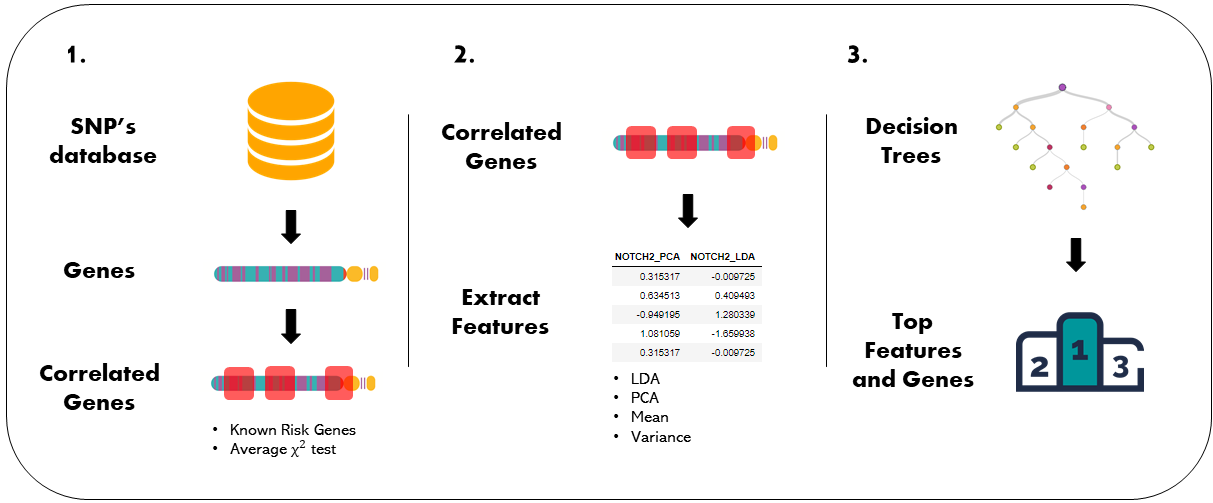
\includegraphics[width=\textwidth]{../images/discussion/feature_diagram.png}
	\caption{Depiction of the pipeline developed to extract important features and discover possible risk genes. On 1. the passage of variants/\gls{SNP}s to finally relevant genes is shown. On 2. it is demonstrated the passage of those genes to features extracted and on 3. the ranking of variables with Decision Trees. } 
	\label{fig:feature_engi}
\end{figure}

After this process, the data was classified using \gls{SVM}s and Extremely Randomized Trees classifiers. It is clear that the \gls{SVM}s with the Gaussian Radial Basis Function kernel were the better performers in every dataset. Also, even though there was a reduction of features to less than 10\% of the original size of the full dataset, only 1\% of accuracy and f1-score were lost. Five-fold cross-validation was then used as a measure to avoid overfitting, and so that we can be more confident in the results. However, the point that provides the most confidence and validity over the pipeline is the 0.94 $\pm$ 0.03 \gls{AUC} with a \gls{SVM} and only known risk genes being used, that shows it can produce accurate classification based on known genes that increase the risk of \gls{T2D}.

At the beginning, as stated before, with the variants and genotypes data, all the classifiers would massively overfit and classify every class correctly, mostly based on incorrect or noisy data. This pipeline, not only provides a way to employ Machine Learning in \gls{GWAS}, but also to correct these issues, be more confident on the data used, and extract novel genes information.

The best \gls{SVM} classifier can also act as risk predictor for this disease, and even output probabilities for a new sample of \gls{T2D} risk. For this purpose, we assume 100 \% to be the highest risk possible, but this is only based on the current data of what the model depicts as the higher risk possible. Nonetheless, these probabilities are only model based, and to develop a truly accurate risk predictor, it is first necessary to get a better understanding of the underlying genetics of \gls{T2D} and make a more truthful representation of the phenotype differences of each patient.

\newpage

\section{Model Shortcomings}

The results of the pipeline are fairly solid and after the dataset quality tests and validation metrics applied, we can be somewhat confident in them. However, there are a few points that the model fails to handle, and some pitfalls that can bias the results. 

The first such point is that the sequencing machines utilized are not the same for the cases and controls groups. The same can be said about the genotyping methods utilized. Nonetheless, it is expected a certain level of confidence and a standardization of the procedures employed, so that the quality of the data is not affected, and the machine from which the genome or exome was sequenced does not matter. To even lessen the variability possibilities, samples from the same ethnicities were used, all to ensure the complete dataset was as reliable as possible. However, the use of samples from only the Iberian Peninsula can also be considered a drawback, as it makes the study plenty restricted in terms of world population reachability. Nevertheless, the pipeline still holds true for any other datasets it can be tested on.

The next shortcoming is relative to the ability of the pipeline to retrieve information of the variants and respective alleles that are responsible for the risk alterations that are seen. This retracing is not impossible, but it was discarded for the advantage of using regions. Since the genes information could be collapsed in single vectors, it was more useful for a machine learning model to access it rather than single variants. The retracing can be performed by looking at the intended original gene and performing association tests, but it is possible that some information is being lost or several variants are needed because of their non-linear interactions. Not providing risk allele information might very well be a pitfall, since many sources expect this kind of information.

Lastly, it is important to discuss the novel risk genes that were identified, their validity, and why are genes non-related to \gls{T2D} considered by the top classifiers. On the first place, since there is no access to the patients data besides their genome, it is not possible to verify if there are any other conditions that might be affecting the results, and if they justify the appearance of many other genes related to risk of other conditions. Nonetheless, only the known risk genes and genes that have no further data available related to disease, already make up for 40\% of the top 25 genes identified in the top 50 features. Even if for a moment we consider those non-related extra genes as noise, it doesn't take away from the fact that the classifiers fare up decently well with only known risk genes. The classifiers look for the best possible data to classify the problem which may lead to usage of noise that fits the classes. To ascertain the validity of some possible novel identified genes, further gene tests would need to be performed.

So far, the results and validation metrics seem to weight up a positive outlook, but further certainty of this pipeline will not be entirely known until further validation can be performed with other \gls{SNP}s or variants datasets.